\documentclass[a4paper,12pt]{article} 
\usepackage{graphicx}
\usepackage{amsfonts}
\usepackage{booktabs}
\usepackage{siunitx}
\usepackage{a4wide}
\usepackage{url}
\usepackage{subcaption} % loads the caption package
\usepackage{float}
\usepackage{amsmath}

\begin{document}

\title{\uppercase{Sorting of many similar lists using memoization techniques}} 
\author{Gonzalo Urroz\\
{\small Master in Computer Science }\\
{\small School of Computer Science and Information Technology, RMIT University } \\
{\small Melbourne, Australia }\\
\and Supervisor: Geoff Leach
}

\date{June 2019}
\maketitle

\begin{abstract}
Sorting is often considered to be the most fundamental problem in the study of algorithms. Some of the most important algorithms are Insertionsort and Mergesort, which have different approaches in solving the same problem and their characteristics makes them suitable for scenarios with lists with small and large amount of elements, respectively. Both algorithms are used in important sorting solutions, Insertionsort is used as part of the standard sorting algorithm implemented in the standard libraries of popular languages such as Java, Python and C++, while Mergesort is used to sort big amount of data in external sorting approaches.\\
Specifically, sorting smaller lists is part of a problem which arises in computer graphics when rendering transparent images using a technique called order independent transparency, or OIT, and involves sorting of millions of small similar lists. The usual approach for this is just to brute force sorting each list one by one, but given the nature of the data, it has been detected that repetition occurs between and within lists. This implies that there may be a chance to store and use the results of previous calculated operations to avoid repetition thus improving performance. This approach is usually known as memoization. 
This research explores several memoization techniques for different cases when there is repetition and similarities in lists, providing what we call the MemoSort and MemoBlockSort techniques which with synthetic data generated specifically to mimic different scenarios, gives performance improvement over brute force sorting starting from 25\% -- 50\% repetition in lists with 128 and 64 elements onwards.

\end{abstract}

\newpage
\tableofcontents
\newpage

\section{Introduction}

Sorting data is one of the most important and studied problems in Computer Science, producing optimised algorithms, data structures and heuristics to solve different range of problems where sorting is involved. This is mostly the case nowadays when gigabytes of information is being produced, stored and analysed in real time and the need for fast sorting is crucial, mainly in sorting big size sets. In general, the algorithms considered for sorting data are the theoretical fastest ones which in an average and worst case scenario have a time complexity of O(n logn), but successfully applying this families of algorithms like Timsort\cite{Timsort} or Introsort\cite{musser1997introspective} (which are implemented in the standard libraries of Java and C++ languages correspondingly) depends greatly in the nature of the data to be sorted, then it is always important to analyse the data to be able to identify which algorithm or approach is best suited. In some cases these algorithms are not sufficient, so different optimising techniques have been produced, for example the usage of parallel programming or using GPU for faster results \cite{satish2009designing}. \\ 

In external sorting, which handles big data sets sorting by using external memory because it is too large to fit in internal memory, involves reading the data not in a linear stream, but in segments of different length that needs to be sorted separately in internal memory and later merged, which can prove to be faster than sorting the whole data as one big set. So applying algorithms that have worse time complexity to each of the segments, like Insertionsort, can perform better than applying Mergesort or other general average case faster sorting algorithm. Big data set sorting optimised algorithms are being researched and published in an international competition \cite{SortBenchmark} \\
\\

\begin{figure}[H]
\centering
\subcaptionbox{Opaque}{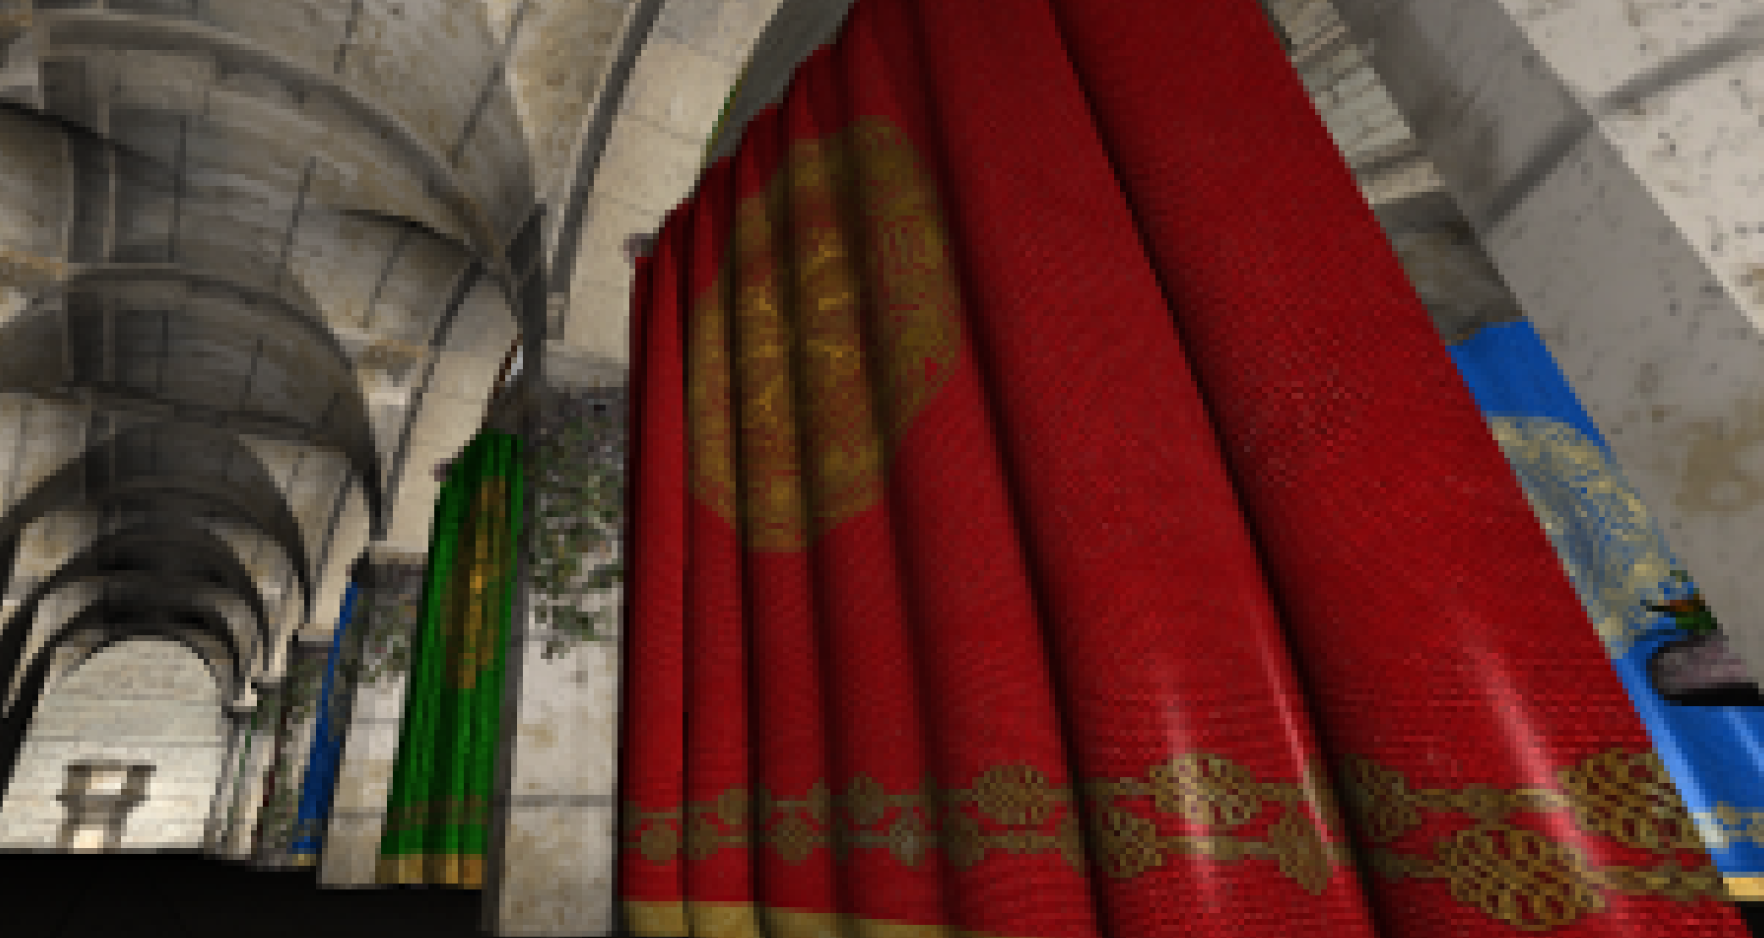
\includegraphics[height=4.0cm,keepaspectratio]{./images/no_transparency.png}}
\hfill % <-- Seperation
\subcaptionbox{Transparent}{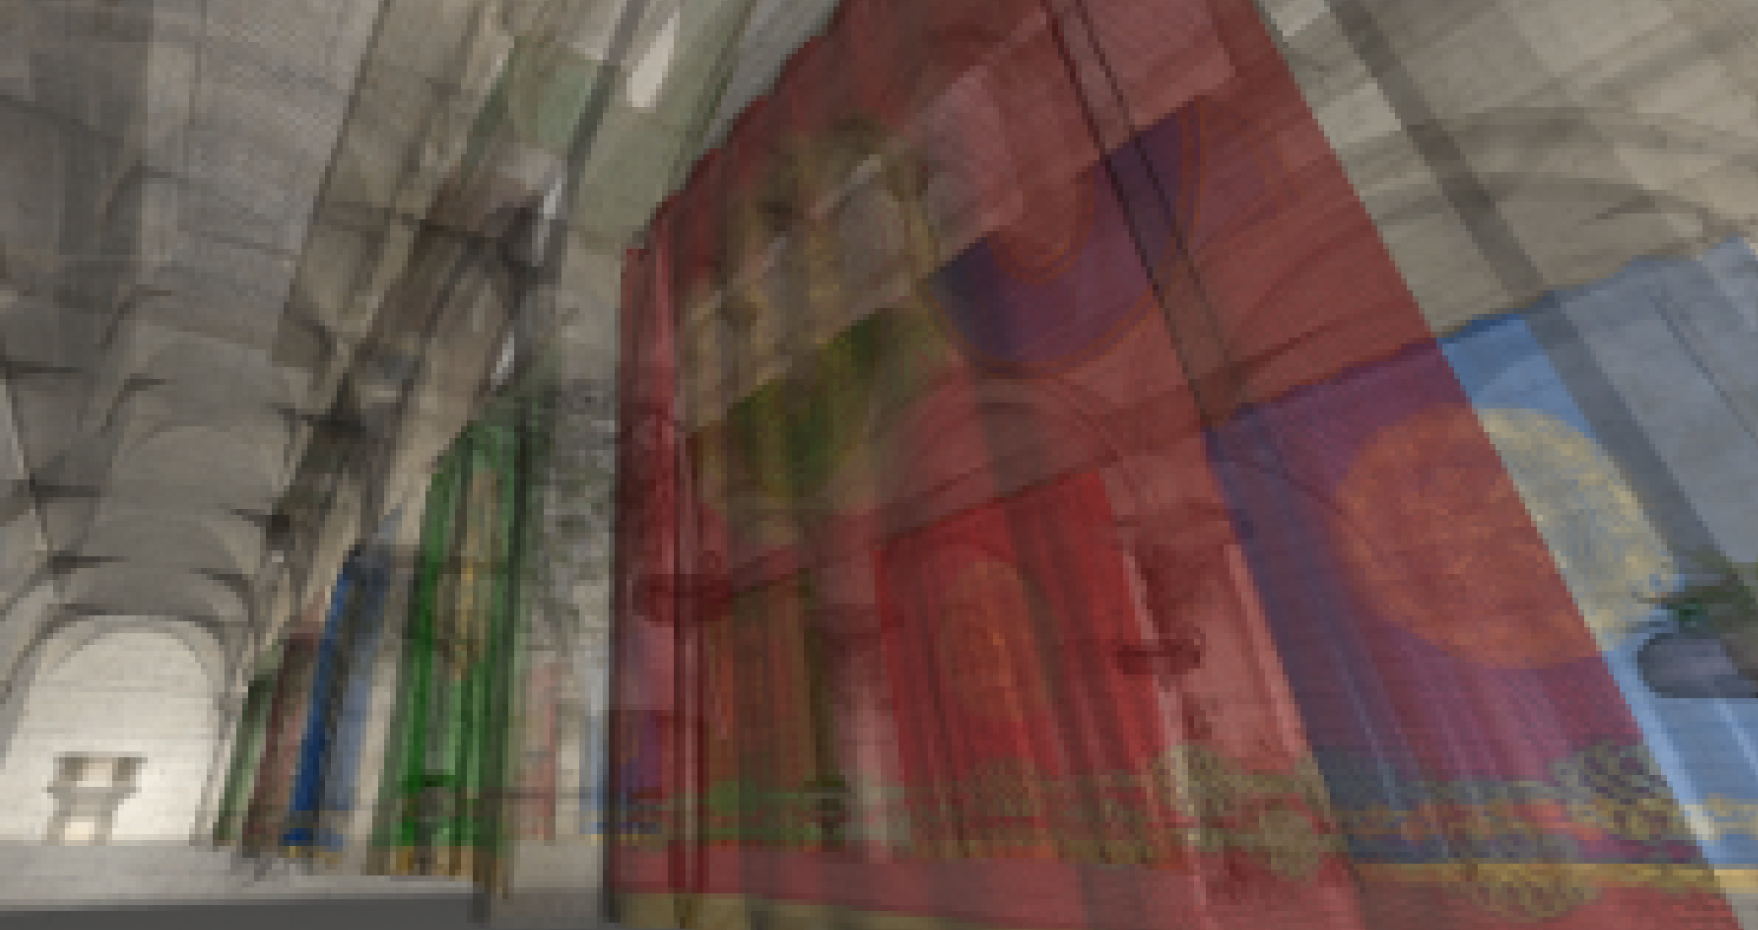
\includegraphics[height=4.0cm,keepaspectratio]{./images/transparency.png}}
\caption{Scene rendered with and without transparency. Taken from \cite{Arch2015}}
\label{fig:Transp}
\end{figure}

A related kind of problem arises in the area of Computer Graphics \cite{Arch2015}, where on the display of computer generated scenes, each object or polygon to be rendered requires multiple computations to be made as quickly as possible to achieve faster graphic rendering, preferably at real time rates. One of these calculations is the transparency value for each polygon in each pixel that screen is displaying (Figure \ref{fig:Transp}). If we considered that nowadays a screen usually holds millions of pixels, therefore millions of calculations need to take place to use a technique called order independent transparency or OIT, which for each pixel must sort each list in depth order before the transparency operation can be performed. The current approach is to sort them by brute force, meaning that all of the lists are sorted independently.

The problem of sorting many small similar lists  has been studied, but not in great length, where most of the solutions involve parallel sorting with multi-threading in CPU \cite{han2002integer} and in GPU \cite{hou2017fast},  implementing hybrid algorithms combining the merging power of Mergesort with the speed of comparison based algorithms, like Insertionsort. 
\\

This research then aims to explore the existance other approaches that could aid in the performance in sorting many similar lists by taking advantage of potential repetition of elements by using memoization, which is a technique to utilise pre-calculated results, in this case the sorted lists. This involves generating a signature to uniquely identify a repeated list, by using the best suited hash function to produce it.
\\

Due to time constraint during the design and development of this study, an abstraction of the original problem is being studied provided with synthetic data, in a way that it allows to simulate the behaviour of this techniques in different scenarios of the similarity between lists. In order to accomplish this, a testbed was developed that allowed the generation of different sets of data, according to the case that needed to be studied to outline the cases in which the potential of memoization on this problem could be of an advantage over the brute force approach.

\subsection*{Research Questions}  \label{researchQuestions}
Memoization (see section \ref{memoHash}) is a optimisation method used in divide and conquer algorithms that consists in the storage of the result of a sub problem for a later utilisation when the same sub problem arises. This gives better performance because it saves the repeated computation of the same sub problem. To achieve this the result must be stored, generally in a lookup table. Dynamic programming uses this kind of memoization to solve problems based in previous results. For our study, we will use a hash table that will hold the signature of a single list as the key and the reference to the sorted list as the value. The aim therefore is not to determine if this techniques optimises the problem, just because it is always faster performing the sorting operation only once, but to determine when does this technique haves better performance given the overhead of calculating the signature and looking up for the presence of the pre calculated value.\\

This work addresses the following research questions:

\begin{itemize}
\item {\bf RQ1:} What are the benefits of utilising memoization techniques to improve repeated list sorting? What are the thresholds at which benefits outweighs costs?
\item {\bf RQ2:} What are the benefit of utilising memoization techniques to improve list sorting when there are repeated blocks of elements within different similar lists? When does it happen?
\item {\bf RQ3:} Which hash function fits better to produce a signature over a list of integers?
\item {\bf RQ4:} What are some possible enhancement techniques that can be applied to improve memoization in sorting?
\end{itemize}

\section{Background}

The problem that is being explored in this research is not the focus of many studies, as there appears to be no direct study on the problem of sorting many similar small lists in the literature. This might be because the problem is not that common or there has not been a need to optimise this process. For this study we consider the different areas that are involved in the objectives or that could be of interest to address the research questions.

\subsection {Sorting Lists}
The kind of algorithms for sorting can be grouped in different categories, with one of them being the internal sort. These are the kind of algorithms that work with all the data within the main memory through out the whole process.

\begin{itemize}
\item {\bf Insertionsort:}  In this category, {\it Insertionsort} is a simple comparison sorting algorithm that has an average and worse case time complexity of O(${n}^2$), but its best case scenario is O(n). Although it has a poor performance for large lists, we will study it because of its good performance in small lists. Being a stable algorithm, mainly because it sorts the elements in place, using only one auxiliary space in memory\cite{knuth1997artInsert}. Compared to other comparison sorting, like Selectionsort and Bubblesort, all have the same time complexity but in practice the efficiency of this algorithm in the average case is superior to the other quadratic algorithms because there are less comparisons steps. Optimisations over this algorithm have been made, such as Shellsort\cite{knuth1997artShell}, Librarysort\cite{bender2006insertion}. Insertion sort is also part of hybrid algorithms such as Timsort\cite{Timsort}, which is the default sorting algorithm in the standard libraries in popular languages such as Java and Python, and  Introsort\cite{musser1997introspective}  which is the default sorting algorithm for languages such as and the .NET framework.

\item {\bf Mergesort:} The approach of this stable algorithm is sorting by divide and conquer, this by merging the result of the subsequent division of the input list into sub lists and recursively dividing and merging them. The standard implementation uses O(n) in space complexity and has average, best and worst case of O(n logn) in time complexity \cite{knuth1997artMerge}. It is suitable for medium and large data set. Multiple optimisations have been made, mainly to reduce the space complexity and the cost of copying \cite{Huang:1988:PIM:42392.42403}.  Other optimisation takes advantage of the nature of the divide and conquer process, by parallelising the execution with multiple threads \cite{chhugani2008efficient} on different architectures and cache optimised versions. Also it is extensible to be used in external sorting.
 \end{itemize}

Even though these are some of the most important, popular and studied algorithms, for some cases there are better tuned algorithms suited for specific data, like the one proposed by \cite{han2002integer}  which sort integers and has {$O(n \sqrt{log log n})$} time and space complexity for average cases.

\subsection {External Sort} \label{ExternalSorting}
External sorting is used when the data to be sorted is too big to fit in main memory so it must be read from the source (network, hard drive) in separate chunks or segments that fits in internal memory. This kind of solution generally apply a hybrid approach in the sorting of the data in memory and merging the final result. 

\subsection{Segmented Sort in GPU} 
In the paper \cite{hou2017fast} a new solution is discussed using the advantage of parallel programming using GPU architecture in order to speed the sorting of segments. The approach proposed is based on data that is naturally segmented, and also the reason why it is interesting for us, the distribution of lengths of this segments tends to smaller ones. The authors then debate over the overhead that using multi threading in GPU and the best way to sort each segment individually. The process that they use is finally clustering each segment in buckets of same size and then sorting each one of them using Bitonic sort \cite{batcher1968sorting} so it can be parallelised in GPU, finally to merge them continuously in memory using GPU registers and warp instructions to speed up the process. It must be noted that their approach does not consider taking advantage from the fact that segments may have some similarities, as is the purpose of this study.

\subsection{Memory Heriarchy}
As much of the literature reviewed exposed, when studying an algorithm not only the time complexity must be taken to account for the performance in speed, because the memory and the operations over it have a great impact on the practical implementation. As Figure \ref{fig:Memory} shows, memory on a modern end user computer follows a hierarchy, where the CPU register is the fastest one, even for multi core architectures. After that comes in the hierarchy the different levels of cache in the CPU which gradually have more capacity but they are more expensive to read and write to, comparing in speed. When the CPU needs to load a particular memory location, it first checks if the required address is already in the cache (checking starts from the lowest level and continues to the highest one). If the required address is absent in the cache, then it must be loaded from the main memory. Such situation is called a cache miss. Sorting algorithm  performance can be improved by aiming to maximise use of cache, reducing expensive cache miss.

\begin{figure}[H]
\centering
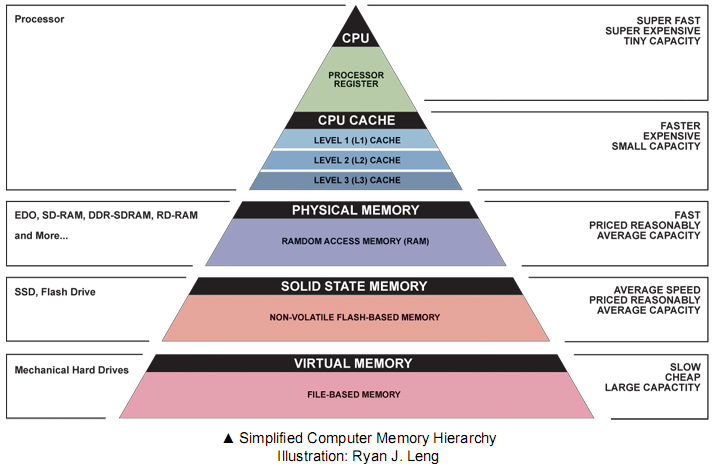
\includegraphics[height=7.5cm,keepaspectratio]{./images/ComputerMemoryHierarchy.png}
\caption{Memory hierarchy. (https://sites.google.com/site/cachememory2011/memory-hierarchy)}
\label{fig:Memory}
\end{figure}

Several modification on known algorithms as Mergesort and Quicksort have been proposed to be {\it cache friendly}, improving the practical performance of such algorithms \cite{lamarca1999influence},  \cite{xiao2000improving}.


\subsection{Memoization and Hashing} \label{memoHash}

Memoization is a concept that has been considered for a long time and has been implemented in different situations \cite{acar2003selective} such as dynamic programming and incremental computation. Most of the applications of this technique are used to prevent repetitions over time, and to make persistent lookup tables \cite{hall1997improving}. This last approach consists in storing a pair of key and value, and being able to quickly fetch the value given the key if it is present in this table. This property is useful when the calculations to be stored as values are uniquely identified by some key. \\

It is then important for this study to explore the creation of this identity key that could allow us to uniquely map a complete list or a sublist or block of the list to be sorted as the key and store the sorted version as the value. \\

Hash functions allow mapping between an arbitrary set of data to a fixed sized data. Hash functions have many uses, from cryptography, file verification to finding duplicates records. A hash function often needs some type of properties depending on the application of it, because what defines a good hash function could be different if it is used to calculate indexes in a database or to use it as a cryptographic signature. \\

A hash function can be defined as universal if the function itself belongs to a family that has the property that the unique value that it evaluates to, h(x), has a probability of 1/M to have two different values x and y to evaluate to the same value, that is h(x) = h(y), which is called a collision. M is the size of all of the possible values the function can return \cite{carter1979universal}.

The classic universal hash function defined in \cite{carter1979universal} is based on a prime number p bigger or equal to M. The constants a and b should be picked from  [1, p-1] and  [0, p-1] respectively, so to define:

\begin{equation}
    h_{a, b}(x) = ((ax + b)  * mod p) * mod M 
\end{equation}


Furthermore a hash function {\it h} is considered strongly universal if the probability of having two different keys, x and y and the hash function for the event h(x) and h(y) is 1/$M^{2}$. In other words, strong universality is that each key is hashed uniformly into M, and that distinct keys are hashed independently, to separate values.\\

When the size of the universe of keys is smaller or equals to the possible outcomes (M), there are ways to construct what is known as a perfect hash function  \cite{sprugnoli1977perfect}, where there is no collisions for any given key.  This might be the best solution to construct a lookup table, or hash table, to be able to apply the memoization technique. Given that the universe of the problem we are exploring consists of a pre defined length of lists and the range of the elements in the lists are limited, there should be a hash function that is perfect for this problem, but the size of M might be too big or the performance of it  could be worse compared to a sufficiently strongly universal or even only universal hash function in this particular study.


\subsection{Compiling versus Interpreting code}
When developing a benchmark framework it is important to consider the precise tools for it. Programming languages have the capability to be interpreted or to be compiled, it all depends if there is a compiler or an interpreter available for the specific language. An interpreter is a program that executes the instruction written in the source code by reading each line of code, translating it to either intermediate code or machine code and executing it, making the source code the actual program. This allows that any machine that has the correspondingly interpreter can run the program, making it inter operable and also easier to debug. Some of the usual interpreters are built for scripting languages, such as Javascript.

On the other hand, compilers produces code from the source code  reading the whole code and transforming it to assembly language, which is then assembled into binary code and packed into a program. This program can only be executed in the same machine architecture in which it was compiled, making it less portable, but generally is faster than interpreting code because each instruction is executed directly, instead of going through the process of being interpreted each time. Languages such as C or C++ are usually compiled.

There is another hybrid approach, where a runtime environment is provided in the machine where the program is set to run. This environment executes code by interpreting it or determining if some part of the code is heavily used, then it compiles it to later execute the compiled code instead of interpreting it. This is called  just in time compiling or JIT. Some of the languages that provides this environments are Java and Python.

\section{Design and Development}
Given the exploratory objective of this research on the feasibility of using memoization on sorting lists, which by itself is a generalisation of a specific problem, the evaluation considers running each sorting algorithm on the same synthetic data set generated specially to understand the behaviour of it in specific cases. The goal is to measure the amount of time taken to sort the full data set, also considering the amount of memory needed to accomplish it.

\subsection{Synthetic Data}

In order for the data set to be representative of the original graphic transparency problem that this study takes inspiration from, the amount of lists correspond to half of what could be the expected amount of data to be processed. This comes from the fact that the sorting of transparency lists needs to be done for each pixel shown in a physical screen, so considering that nowadays most screens have a what is called full high definition (FHD) resolution, which display a resolution of 1,920 x 1,080, there is around 2 millions pixels to sort. For the purpose of this study  we will use half of the amount of available pixels (approximately 1 million) because it provides a good enough representation of a real case scenario but it still allows to run test in a environment without exceeding system memory or CPU specification.

Each of the million lists to be tested is generated to hold uniformly distributed random generated integer numbers that range between 0 and RAND\_MAX using a C++ program. RAND\_MAX may depend on the particular implementation, but is normally  $2^{31}$-1, i.e. 2,147,483,647 on a 32 bit machine, just  to have a big enough pool to distribute it through the different lengths that are tested, which vary between cases. To generate the baseline on run time between sorting algorithms and also compare them using the new algorithms to use memoization in order to answer RQ1, the length of the lists considered were from 16 integers to 512. For RQ2 to be answered, this is sorting blocks within the lists, a larger length of the lists is needed because of the expected overhead that reading and merging blocks or sublists brings, so for smaller lists no better performance is expected given that brute force is already fast enough, so increasing the length size permits for an actual appreciation of what could be the benefits of applying this technique.\\

Finally, each list data is generated according to the scenario that it is being tested. Given that for RQ1 and RQ2 the behaviour that it is studied is on repeating list and similar list, it is then necessary to state how many or proportions of repeated lists and how similar they are. 

\subsection{Test Cases}

For RQ1 different scenarios will be tested on each list length size. Each scenario is as follow:
\\

\begin{table}[H]
\centering
\begin{tabular}{|r|l|}  \hline
	{$Repetition (\%) $} & {$Description$}  \\  \hline
	100 & Only one original list \\
	75 & 250,000 original list \\
	50 & 500,000 original list \\
	25 & 750,000 original list \\
	0 & All list are different  \\  \hline
\end{tabular}
\caption{RQ1 test bed}
\end{table}

For RQ2 the different scenarios are the following:
\\
\begin{table}[H]
\centering
\begin{tabular}{|r|l|}  \hline
	{$Repetition (\%)$} & {$Description$}  \\  \hline
	100 & Only one  original block \\
	75& 250,000 original blocks   \\
	50& 500,000 original blocks \\
	25& 750,000 original blocks \\
	0 & All blocks are different \\  \hline
\end{tabular}
\caption{RQ2 test bed}
\end{table}

For each of these scenarios, three blocks sizes will be tested,  8, 16 and 64. The idea is to study the impact of the block size to determine how it affects in the performance but only a subset of them are chosen because choosing a higher block will convert it into a RQ1 scenario and because of time constraint not all possible combinations can be tested. \\

The testbed used is a 2017 MacBook Pro, with a 2.3 GHz Intel Core i5 and 16 GB 2133 MHz LPDDR for physical memory. Compiled with Apple LLVM version 10.0.1 (clang-1001.0.46.4) in macOs Mojave 10.14.4, with 32K/32K Level 1 cache.

\subsection{Hash Function}

In order to consider which hash function to implement, the universe of possible inputs has to be considered. We are only working with sets of integers with elements between 0 and RAND\_MAX, and each list (or a block of it) is a key or input for the hash function. 
Then the size of the universe of keys is the combination of the range of integers over the size of the lists $\binom{RAND\_MAX}{Max list length} $, which in the environment where the test bed will be run, where max list length is 512, it is in the order of $10^{3611}$.

Given this universe size, considering a perfect universal hash function is impossible because the potential hash table needs $10^{3611}$ elements to map to. In consequence, a strongly universal hash function will be considered.

As reviewed by \cite{thorup2015high}, one of the fastest techniques to construct a strongly universal hash function for an integer set is to multiply and shift pairs of elements, given the following formula:

\begin{equation}
	h_{a_0,a_{d-1},b} (x_0, x_{d-1}) = \Bigg(\Bigg( \sum_{i=0}^{d/2} (a_{2i} + x_{2i+1})  (a_{2i+1} + x_{2i})\Bigg)  + b\Bigg) [W-l, W).
\end{equation}

Where {\it d}  is the length of the set and is assumed to be even. The set {\it a} is a set of uniformly random distributed integers in the  range $[0,2^w]$ where w is the number of bits of the keys, {\it b}  is just a constant in the range $[0,2^w]$. The seed {\it l}  is the bits of the hash value. {\it W}  is at least the sum of w + l -1 or higher. \\
Then the hash function is named {\bf PairMultiplyShift}, and has the following pseudo-code:

\begin{figure}[H]
\begin{verbatim}
int hash(int[] data, int l, int[] a, int b, int w, int d) {
    hash = 0;
    for(int i = 0; i < d/2; i++) {
        pairResult =  (a[2i] + data[2i+1]) * (a[2i+1] + data[2i]);
        hash +=  (pairResult + b) >> (w-l);
    }
    return hash;
}
\end{verbatim}
\caption{Proposed PairMultiplyShift hash function}
\end{figure}

For our case, the keys used are 32 bit integers (4 bytes) and the algorithm involves multiplication then we need to handle 64 bits results, so in order to maintain a low probability of collisions and taking advantage that the 64 bit multiplication automatically discards overflow,  the hash value is defined as 64 bits (8 bytes)
\\

It is then established that this kind of hash function has a time complexity of O(n) and space complexity of O(l). For educational purpose and to understand the impact of choosing the correct hash function, other hash functions are also tested, even though it is known before hand that some of them are not the best solution to the problem.

The following hash function are compared:

\begin{itemize}

\item {\bf MD5:} This is a cryptographic function \cite{rivest1992md5} which is no longer regarded secure \cite{wang2005break}.  The implementation is given by the standard C++ library {\it CommonCrypto}.

\item {\bf PrimeAdd:} The naive approach of just adding the value of each element and multiplying by a prime number. The objective is to do simple operations, multiplication and addition, and exploiting the know properties of prime numbers of producing number with less common factors. \\ 
The hash function is:

\begin{figure}[H]
\begin{verbatim}
int hash(int list[], int length) {
 long hashVal = 17;
    for(int i = 0; i < length; i++) {
        hashVal = hashVal * 19 + list[i];
    }

    return to_string(hashVal);
}
\end{verbatim}
\caption{Proposed PrimeAdd hash function}
\end{figure}
 

\item {\bf MurMur3:} A non-cryptographic hash function suitable for general hash-based lookup. Implemented based on the source code available online \cite{MurMur3}. This hash function works by rotating, shifting and xoring chunks of bytes. It provides 3 methods, 1 for hash values of 32 bits and 2 for 128 bits (for x86 and 64 bits architectures). The one used is MurmurHash3\_x64\_128, but 64 of the 128 bits are discarded to maintain the same value to compare to other functions.

\end{itemize}

\subsection{Implementation of Insertionsort and Mergesort} \label{SortingImplementation}
It is important to discuss the implementation of the sorting algorithms as it impacts directly on performance and extensibility.

For Insertionsort, the implementation used is the straight forward iterative approach, comparing tuples starting from the second position and moving to the end of the list. The implementation is as follows:

\begin{figure}[H]
\begin{small}
\begin{verbatim}
void InsertionSort::sort(int list[], int length) {
    int value;
    int i, j;
    for(i = 1; i < length; i++) {
        value = list[i];
        j = i-1;
        
        while (j >= 0 && list[j] > value) {
            list[j+1] = list[j];
            j = j-1;
        }
        list[j+1] = value;
    }
}
\end{verbatim}
\end{small}
\caption{Insertionsort implementation}
\end{figure}


The case for Mergesort is more interesting, because the natural approach is to have depth first  recursive calls. However, using a bottom up approach is faster, which is an iterative double loop that operates in place and merges the arrays in pair, doubling the range of each tuple in each loop. A slight improvement is made by using a temporary array to merge the sublists outside the merge step, saving some copy operations. The advantages for this choice of implementation is to avoid the recursive function call overhead and the ability to access in place to all elements, which gives the opportunity for further modifications when considering memoization over the algorithm.

\begin{figure}[H]
\begin{small}
\begin{verbatim}
void MergeSort::mergeSort(int list[], int tmp[], int length) {
   for(int size = 1; size < length; size = 2 * size) { 

       for(int iStart = 0; iStart < length; iStart += 2 * size) {
           int left = iStart;
           int middle = iStart + size;
           int right = iStart + (2 * size);

           merge(list, tmp, left, middle, right);
       }
       
       for(int i = 0; i < length; i++) {
           list[i] = tmp[i];
       }
   }
}

void MergeSort::merge(int list[], int tmp[], int iLeft, int iMiddle, int iRight) {
  int i = iLeft;
  int j = iMiddle;
  int globalIndex = iLeft;

  while (i < iMiddle || j < iRight) {
      if ( i < iMiddle && j < iRight ) {
          if ( list[i] < list[j] )
              tmp[globalIndex++] = list[i++];
          else
              tmp[globalIndex++] = list[j++];
      }
      else if ( i == iMiddle )
          tmp[globalIndex++] = list[j++];
      else if ( j == iRight )
          tmp[globalIndex++] = list[i++];
  }
}
\end{verbatim}
\end{small}
\caption{Mergesort bottom up implementation}
\end{figure}

\subsection{Hash table: Unordered map} \label{hashTable}
As stated earlier, the selected underlying hash table used to store the signature is the one offered as part as the containers library in C++ named unordered\_map, which is a structure that holds the pair (key, value) and it has O(1) in the average case for the search, insert and delete operation.

This hash table expands automatically because it keeps count of the number of items stored and grows its size and rehashes all elements when it reaches a defined load factor, which is the ratio between the number of elements and the size of the hash table. 

\begin{figure}[H]
\centering
\subcaptionbox{Insertion}{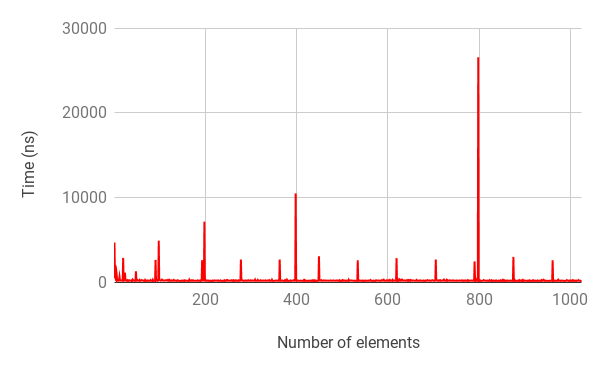
\includegraphics[height=4.5cm,keepaspectratio]{./images/insertHashTable.png}}%
\hfill % <-- Seperation
\subcaptionbox{Look up}{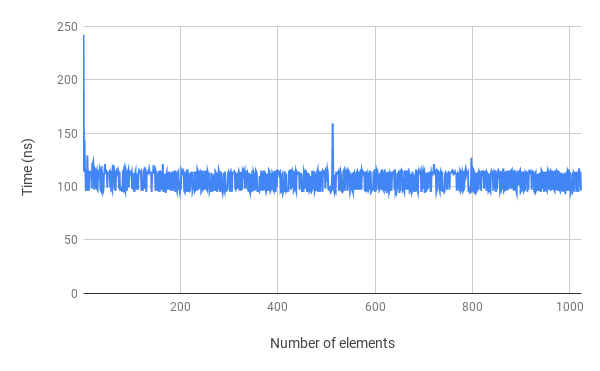
\includegraphics[height=4.5cm,keepaspectratio]{./images/searchHashTable.png}}%
\caption{Unordered map operations}
\label{fig:hashTableFig}
\end{figure}

Empirically the operations of insertion and look up values can be viewed in Figure \ref{fig:hashTableFig}, where 1024 random integers were inserted and immediately searched. The insertion operation have spikes that are bigger as the hash table is filled, which is explained by the resizing process explained before. 

It can be viewed that both insertion and search operation generally maintains a constant time in average, but looking up for one element is order of magnitude faster than inserting. \\

In order to avoid this costly resize operation, it is a good practice to reserve the expected size of the hash table before inserting elements. 

\subsection{MemoSort for Repeating Lists}
To be able to take advantage of the possible repeating nature of the problem being studied we use the described hash table and hash function to implement a memoization technique. We propose \textbf{MemoSort} which is the algorithm being studied to establish its real benefits, and its outline can be viewed in Figure \ref{fig:MemoSortDiagram} and Figure \ref{fig:MemoSortDiagramHash}.

\begin{figure}[H]
    \centering
     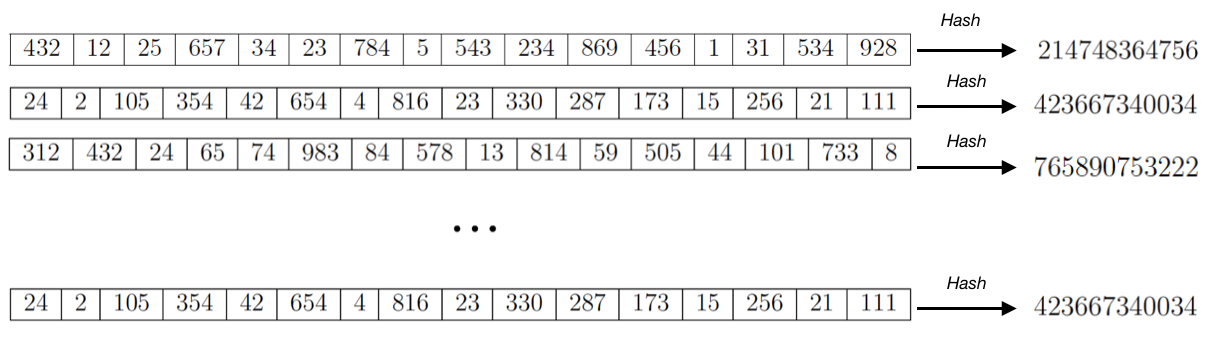
\includegraphics[height=4.5cm,keepaspectratio]{./images/MemoSortDiagram.png}
    \caption{Signature calculation for each list}
    \label{fig:MemoSortDiagram}
\end{figure}

\begin{figure}[H]
    \centering
     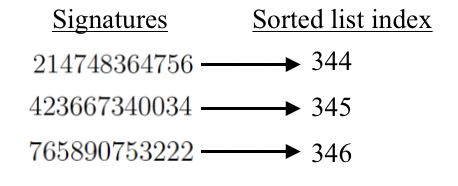
\includegraphics[height=3cm,keepaspectratio]{./images/hashTableDiagram.png}
    \caption{Hash table holding signatures as value and reference of the original list as value}
    \label{fig:MemoSortDiagramHash}
\end{figure}

The algorithm is defined by the pseudo code that can be seen in  Figure \ref{fig:MemoSortAlgo}.

\begin{figure}[H]
\begin{small}
\begin{verbatim}
for(j = 0; j < listLength; j++) {
    signature = hashFunc.hash(lists[j]);  // Generates signature for list
    sortedListIndex = hashTable.find(signature) // Look up signature in hash table
    
    if(sortedListIndex not found) // New list to be sorted
         sortFunction.sort(lists[j]); // Sorts list
         hashTable.insert(signature, j); // Stores the reference to the sorted list
     } else  // List already sorted
        lists[j] = lists[sortedListIndex] // Copy sorted list
}
\end{verbatim}
\end{small}
\caption{MemoSort pseudo algorithm}
\label{fig:MemoSortAlgo}
\end{figure}

The theoretical behaviour for each of the sorting algorithm gives us an idea on the amount of overhead that the construction and  execution of the look up in the hash table has to take. 

For Insertionsort, the worst time complexity is O($n^2$), where n is the length of the list and if M is the total number of lists to sort in the brute force case, and M$'$ the amount of unique lists to sort when using memoization, then it follows that:

\begin{equation}
M * O_{sorting}(n^2)  \geq M' * O_{sorting}(n^2)  + Overhead
\end{equation}
Which implies
\begin{equation}
(M - M') *  O_{sorting}(n^2)  \geq Overhead
\end{equation}

As the memoization technique involves calculating the signature for each list, looking up each, and insert only the ones that are unique, then:

\begin{equation}
Overhead =  M * O_{hashing} + M * O_{lookup} + M' * O_{insert}
\end{equation}

Accordingly the implementation of the hash table then has to be constant for both the search of a key and in the insertion of a new tuple. Other operations as delete or edit are of no concern because they do not apply for the use of this memoization technique. Then constructing the hash table is a matter of using the correct data structure. For this case the choice was to use an unordered map (see  section \ref{hashTable}). Other options involves the use of trees, which have O(n logn) operations. Also it is assumed that the hash function utilised is O(n). 

In consequence for the memoization technique to be beneficial it must stand that:

\begin{equation}
(M - M') *  O_{sorting}(n^2) \geq M * O_{hashing}(n)+ M'
\end{equation}

From this, the following cases can be defined:
\begin{itemize}
\item {\bf All lists are the same:}  This means M$'$ = 1, holds clearly that (M - 1) *   $O_{sorting}(n^2)$   $\geq M *O_{hashing}(n)$ + 1
\item {\bf None of the lists are the same:} This means M$'$ = M. Then there is no benefit as 0 $ \geq M * O_{hashing}(n)$ + M is not true if M $>$ 0
\end{itemize}

The same analysis can be made for the case of Mergesort where sorting is for worst case is O(nlogn). \\

\subsection{Optimised MemoSort for Repeating Lists} \label{OptMemoSort}
The intuition to this approach comes from the fact that when sorting there is the need to visit each element at least once, as is the same in the current approach of calculating the signature, so merging both processes may result in a faster algorithm. Previously, first the signature was calculated reading the whole list, and if it was a new list, then it was sorted by reading the whole list again.
The new approach is that for each list the hash table holding the current calculated signatures is passed as a reference to the sorting method and queried as soon as the signature is calculated. If the signature is not present, the signature is stored in the hash table with the reference to the ordered list. \\

To be able to calculate the signature, the hash function needs to be able to construct the hash value in an incremental way. For this reason is why neither {\it Murmur3} or {\it PairMultShift}  are suitable because they do not operate with only one element at a time, so the chosen hash function is {\it PrimeAdd} which behaves in a similar way to the named hash functions but operates on one element at a time.

The modifications made to Insertionsort are minimal, given that calculating the signature is possible only when the last element is read, which happens at the end of the algorithm.

Different is the case of Mergesort where after the first pass of the merge step all elements have been visited and the signature can be calculated, thus saving all the subsequent merging steps.

\subsection{MemoBlockSort for Similar Lists} \label{MemoBlockSort}
A broader case can be considered as a possibility to apply memoization techniques, where lists are different from others but parts or {\it blocks} repeat between the lists. The proposed algorithm, {\it MemoBlockSort}, works in a similar way to the proposed  {\it MemoSort} but instead of calculating signatures for whole lists, it uses blocks of elements of a predefined length in each list as it can be seen in Figure \ref{fig:MemoBlocSortDiagram} and the unique signature of each block is then calculated as seen in Figure \ref{fig:MemoBlocSortDiagramHash} . Then after the process of checking existence, sorting and inserting in the hash table, a third step takes place, which is the merging of the sorted blocks to re generate the list in a sorted order.\\

\begin{figure}[H]
    \centering
     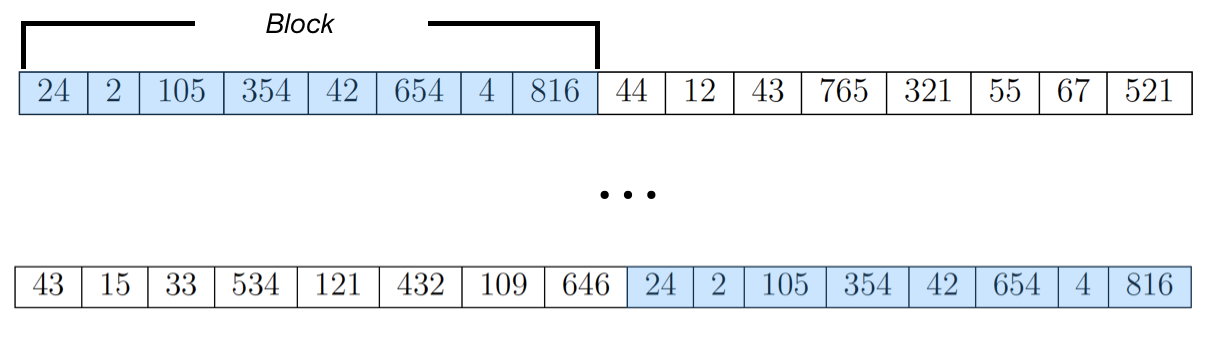
\includegraphics[height=4cm,keepaspectratio]{./images/MemoBlockSort.png}
    \caption{Blocks of size 8 in a 16 size list repeated within different lists}
    \label{fig:MemoBlocSortDiagram}
\end{figure}

\begin{figure}[H]
    \centering
     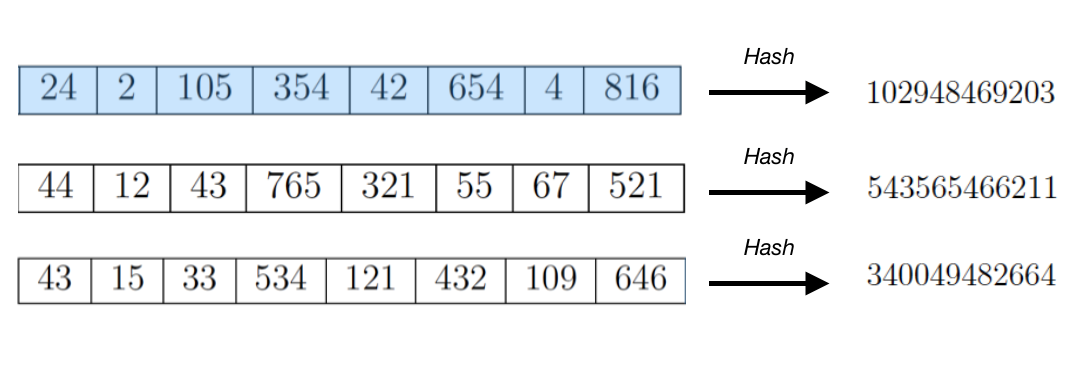
\includegraphics[height=4cm,keepaspectratio]{./images/MemoBlockSortHash.png}
    \caption{Unique blocks signature calculated}
    \label{fig:MemoBlocSortDiagramHash}
\end{figure}

In order to test this approach, the list need to be constructed in a special way, because when we talk about repetition, is how many times a specific block is repeated. This repetition can happen in many ways, distributed between different list, or the simpler way when the repetition is in the list itself. So all blocks are distributed in equal manner in each list.\\

Each of the unique blocks are generated with uniform random integers and the rest of the lists is filled with uniform random integers. This generates lists that do not have a uniform random distribution, given the repetition of blocks. This characteristic impacts in the sorting performance of Insertionsort and Mergesort, so for each scenario the brute force sorting of the whole list is calculated to be able to compare correctly. 

The test bed to determine the behaviour of this approach includes different block and list sizes, comparing both for Insertionsort and Mergesort. \\

The first overhead that can be distinguished is the amount of possible signatures created, if L is the length of the lists, M the amount of lists, B the length of the blocks and U the factor of repetition, the amount of signatures calculated is given by the equation :

\begin{equation}
Number of signatures \leq  M * (L / B) * U
\end{equation}

Then the overhead is affected by the factor (L/B) and U, which not only impacts the size of the hash table, but also the number of iterations and reading and writing of data. So it is expected that the overhead of managing blocks will make this approach less optimal compared to the previous scenario of just sorting repeating lists, but at the same time broadens the applications of this memoization technique.

\subsection{Optimising MemoBlockSort with 2-way-merging}
One of the main optimisations to MemoBlockSort is in the process of merging the blocks to produce the sorted result of the original list. The procedure includes taking all the references to the different already sorted blocks in the original list and merge them. The naive way of doing this is just copying each block back to the list in the sorted order, and later run a the sorting algorithm to this semi ordered list to sort it completely. Clearly this approach works, but it is similar to just sort the list without the whole process.

So a better way to merge this comes from the Merge phase of the Mergesort algorithm (see section \ref{SortingImplementation}), which merges the different sublists by pairs. Similarly, the approach taken here is to iteratively merge each block with a temporary list, and by this merging just two sub lists at a time. At the end of all blocks merging, the temporary list is copied to the original list.

\subsection{Optimising MemoBlockSort with k-way-merging}
Another way to merge the blocks can be found in external sorting problems (see section \ref{ExternalSorting}) which involves merging k sublists into a new list, in this case merge all the blocks where k =  (L/B) into the original list.\\

The procedure for this is taking advantage that the blocks are already sorted, so for each position in the original list the minimum value is calculated as described in Figure \ref{kWayMerge}.

\begin{figure}[H]
\begin{small}
\begin{verbatim}
// Iterates over each position in the original list
for(i = 0; i < listLength; i++) {
    int minVal = MAX_VALUE; // Sentinel value for initial comparison

    for(int k = 0; k < numberOfBlocks; k++) { // Iterates over each block
        int lastIndex = blockLastIndex[k]; // Gets the last position visited in that block
		
       if(lastIndex < blockLength && minVal > blocks[k][lastIndex]) {
            minVal = blocks[k][lastIndex]);
            blockLastIndex[k] = lastIndex++;  // moves the position of the index
       }
    }
    originalList[i] = minVal;
}
\end{verbatim}
\end{small}
\caption{K-way merge}
\label{kWayMerge}
\end{figure}

\section{Results}

\subsection{Benchmarking}

The first activity that was developed was to design and build a software framework that could guarantee correct and trustworthy calculation of the execution of certain algorithms. The first approach was to develop the software in Java language version 8, but it proved to be a not so reliable language for benchmarking given that the Java Virtual Machine environment on which the program runs, uses JIT  compilation and handles memory through a garbage collector in a unpredictable way, thus when running experiments results varied to a large degree. The first measure to mitigate this was to run each test ten times and calculate an average on the result. Also, to prevent the compilation of code throughout the test, the code had to be {\it warmed up} by executing it a number of times so it would be forcefully compiled. 

Even after taking these measures, the tests took a long time to run, and the results were still not as solid as required to confidently compare algorithms. For that reason, the code was re written in C++. With this new code the test where  executed and it prove to give more concise and uniform results. This allowed to execute the test a couple of times without having a big difference, producing consistent results in overall, so the measures presented are the execution of a single test.

\subsection{Mergesort versus Insertionsort}

\begin{figure}[H]
    \centering
     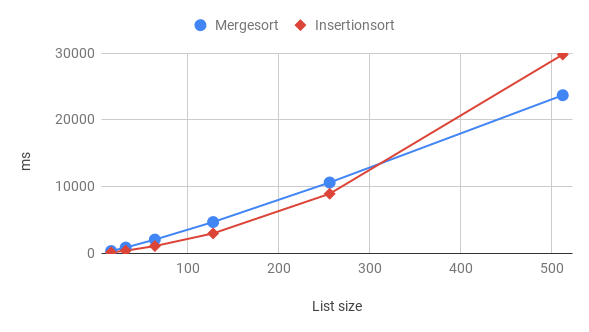
\includegraphics[height=8cm,keepaspectratio]{./images/InsertionvsMerge.png}
    \caption{Insertionsort versus Mergesort sorting 1 million lists}
    \label{fig:InsrtVsMerge}
\end{figure}

The first experiment executed was to compare algorithms Insertionsort and Mergesort given the synthetic data set created, sorting a million lists in different , using the same parameters for each one. As the literature confirms, Insertionsort has a better performance on smaller length list. By using the parameter $-O2$ to compile the code with level 2 optimisation, better results are obtained and Insertionsort sorts in less time up to length of 256 elements. After this list length, Mergesort has a better performance.

The time taken to sort the lists in milliseconds is displayed in Figure \ref{fig:InsrtVsMerge}. Only the average case (random order) for both algorithms is displayed and they exhibit the expected behaviour, this is  O(${n}^2$) for sorted array in Insertionsort and O(n logn) time complexity for Mergesort.  But for smaller lengths as 16 and 32 elements, Insertionsort is 2 times faster than Mergesort but at 256 only 0.2 times faster. 

This is explained because Insertionsort performs less operations and most importantly has less read and write operations over the array. In contrast, Mergesorts reads and writes through the data for each merge, making it more expensive to sort when the overhead of this operations takes almost all the time of the sorting, which happens when the amount of elements is small.

\subsection{Hash Functions}

\begin{figure}[H]
    \centering
    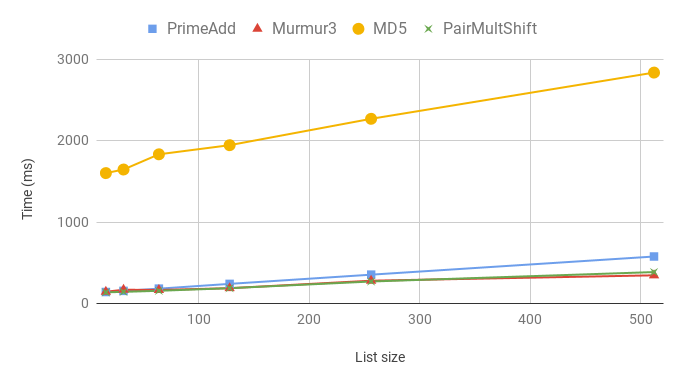
\includegraphics[height=8cm,keepaspectratio]{./images/hashes.png}
    \caption{Hash functions time calculating signature over 1 millions lists}
    \label{fig:HashesFunc}
\end{figure}

From Figure \ref{fig:HashesFunc} is it clear that all hashing function have a linear behaviour as expected, but they do show performance differences between them. It is obvious that MD5 is not a viable hash function to use for this study because of the time it takes compared to the other functions, being near an order of magnitude of difference, i.e. 10x. This confirms that this functions is not designed for use in a hash table.

Then when comparing the other three hash functions, {\it PrimeShift} hash function behaves as wells as the others two, but it begins to be slower after the array length is bigger than 64 elements. The difference continues to increase as there are more elements in the lists.

Both {\it Murmu3} and {\it PairMultShift} behave in a similar way, growing by a really small amount and having a small difference between them, that could be part of the randomness of the tests. Both approaches are radically different but behaves as well for list of integers.

It must be stated that all of the hash functions presented 0 collisions for each of the runs.\\

These result shows that the cost of hash function can be considered small if compared to operations such as sorting the list, even more for bigger list sizes like 256 and 512, where the time to hash the list is almost the same as for smaller list. For smaller sizes it still behaves better than sorting but the cost is comparable for sizes such as 16 and 32 elements.

\subsection{Memoization Costs}

In order to better compare the performance of the memoization techniques, a base cost must be stablished in the use of a hash table, by determining the time spent inserting and searching from it. An experiment was conducted to determine how much time did it take in the operation of inserting the expected amount of signatures, and how much time it takes to search for each signature while the hash table was being populated. \\

\begin{table}[H]
\centering
\begin{tabular}{|c|c|c|c|c|}   \hline
	{$Operation$} & {$0.25M$} & {$0.5M$} & {$0.75M$} & {$1M$} \\  \hline
	Look up & 61 ms & 127 ms& 199 ms & 270 ms\\ 
	Insertion & 90 ms & 173 ms& 269 ms& 363 ms\\  \hline
\end{tabular}
\caption{Hash table operation time}
\label{ref:MemCostTable}
\end{table}

The readings shown in Table \ref{ref:MemCostTable} are the sum of the time taken by each operation while constructing the hash table. Both operations increased in time with the number of elements stored in the hash, inserting being around 20\%--30\% more expensive than reading from the hash table. Has to be noted that in MemoSort algorithm the operations are not executed the same number of times, except in the case where there is no repetition, because look up is executed for the total amount of lists and insertion only happens when the signature is not  already present, which depend on the repetition of lists.

\subsection{MemoSort for Repeating Lists}

The following result represents the test over uniformly distributed random data after applying the memoization technique using a hash table, and utilising the proposed hash function {\it PairMultShift}  to generate the signature of each of the unique list. \\

\begin{figure}[H]
    \centering
    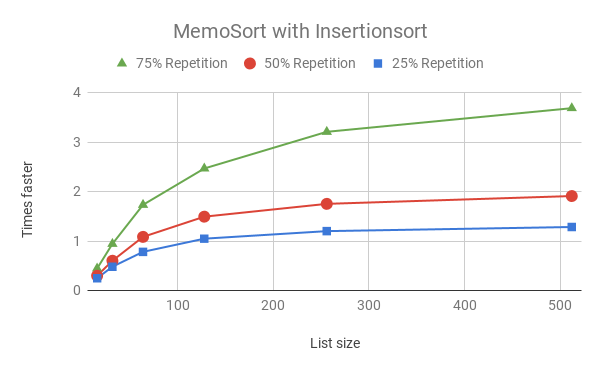
\includegraphics[height=8cm,keepaspectratio]{./images/MemoSortIns.png}
    \caption{Times MemoSort is faster than brute force Insertionsort }
    \label{fig:MemoSortInsGraph}
\end{figure}

\begin{table}[H]
\centering
\begin{tabular}{|r|r|r|r|r|r|r|}   \hline
	{Length}  & {$100\%$} & {$75\%$} & {$50\%$} & {$25\%$} & {$0\%$} \\  \hline
	16  &0.982& 0.445 & 0.299  & 0.249 &  0.213 \\ 
	32 & 2.155 & 0.944 & 0.602 &  0.482 & 0.402 \\ 
	64 &  5.989 & 1.734 & 1.085 & 0.782 & 0.637 \\ 
	128 &14.587 & 2.469 & 1.494 & 1.049  & 0.819 \\ 
	256 & 28.572& 3.211 & 1.754 & 1.202 & 0.915 \\ 
	512 & 82.792& 3.690 & 1.912 & 1.285 & 0.970 \\  \hline
\end{tabular}
\caption{MemoSort speed factor using Insertionsort with different repetitions}
\label{fig:MemoSortInsTable}
\end{table}

The results displayed in Figure \ref{fig:MemoSortInsGraph} shows the performance comparison between different scenarios of repetition, leaving out the border cases of 0\% and 100\% repetition as they behave as expected and their results distorts the graph, nevertheless they can be viewed in Table \ref{fig:MemoSortInsTable}. \\

The results shows the times MemoSort is faster than sorting by brute force all lists. We can see that there is a severe penalty for using this approach in small lists length, like 16 and 32 element for Insertionsort. There starts to be an improved performance after lists with length of 128 for most repetition scenarios, but at 64 there is an improvement if the data is repeated between 50\%--75\%. This is  mainly because the sorting performance below this length surpass the overhead of calculating and looking up the signature of the list. \\
As it is expected, when there is no repetition, there is only overhead in applying this approach. The trend tends to be that the bigger the list length and higher repetition, the more performance improvement there is, as would be expected.\\

The same behaviour is shown for Mergesort in Figure  \ref{fig:MemoSortMergeGraph} , but the performance improvement is not given much by the length of the list, as only for the amount of repetition given that the increase or decrease is not so drastic as with Insertionsort. The border cases of 0\% and 100\% repetition can be viewed in Table \ref{fig:MemoSortMergeTable}, where it shows only worst and better performance respectively for each lists length.

\begin{figure}[H]
    \centering
    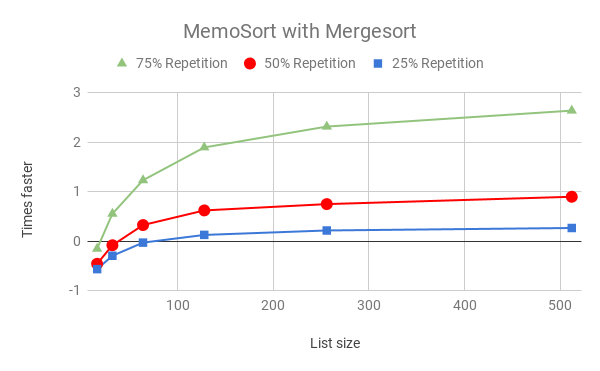
\includegraphics[height=8cm,keepaspectratio]{./images/MemoSortMerge.png}
    \caption{Times MemoSort is faster than brute force Mergesort }
    \label{fig:MemoSortMergeGraph}
\end{figure}


\begin{table}[H]
\centering
\begin{tabular}{|r|r|r|r|r|r|r|}   \hline
	{Length} &  {$100\%$} & {$75\%$} & {$50\%$} & {$25\%$} & {$0\%$} \\  \hline
	16 & 2.116&0.845 & 0.540 & 0.434 &0.356\\ 
	32 & 5.262&1.554 & 0.916&0.703& 0.568\\ 
	64 & 10.937 &2.232&1.324&0.969&0.753\\ 
	128 & 20.636&2.895&1.621&1.125&0.865\\ 
	256 & 35.089&3.317&1.748&1.215&0.919\\ 
	512 &  58.978&3.640&1.897&1.265&0.958\\  \hline
\end{tabular}
\caption{MemoSort speed factor using Mergesort with different repetitions}
\label{fig:MemoSortMergeTable}
\end{table}

\subsection{Optimised MemoSort for Repeating Lists}

\begin{figure}[H]
    \centering
    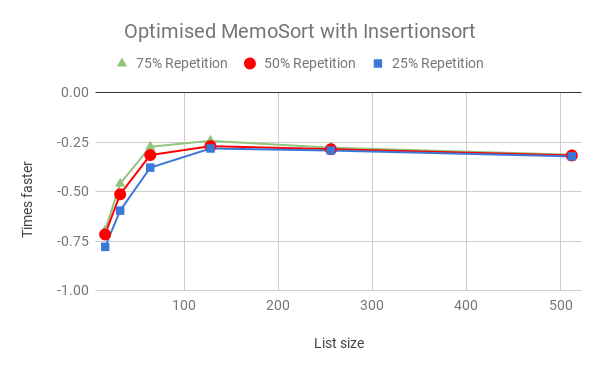
\includegraphics[height=8cm,keepaspectratio]{./images/OptMemoSortIns.png}
    \caption{Times Optimised MemoSort is faster than brute force Insertionsort}
    \label{fig:OptMemoSortInsGraph}
\end{figure}

\begin{table}[H]
\centering
\begin{tabular}{|r|r|r|r|r|r|r|}   \hline
	{Length} & {$100\%$} & {$75\%$} & {$50\%$} & {$25\%$} & {$0\%$} \\  \hline
	16 &0.802&0.303 & 0.284 & 0.221 & 0.196\\ 
	32 &1.263&0.541 & 0.487& 0.404& 0.363\\ 
	64 &1.269 &0.728&0.685&0.621& 0.593\\ 
	128 &0.898&0.757&0.730&0.719 &0.708\\ 
	256 &0.753&0.723&0.715&0.708&0.704\\ 
	512 & 0.688&0.687&0.683 &0.678 &0.681\\  \hline
\end{tabular}
\caption{Optimised MemoSort  speed factor using Insertionsort with different repetitions}
\label{fig:OptMemoSortInsTable}
\end{table}


As discussed in section \ref{OptMemoSort} and shown in Figure \ref{fig:OptMemoSortInsGraph}, there is no improvement from just running the optimised version of MemoSort on the different scenarios. This is because this algorithm does not apply the full potential of memoization as it only looks for previous sorted lists only at the end of the process of sorting each list, adding the overhead of the memoization technique to the time required to sort the rest of the list. \\

For Mergesort the case is different, as shown in Figure \ref{fig:OptMemoSortMergeGraph}, there is improvement compared to just brute force sort all the list as well as just applying MemoSort. Interestingly, it does not improve as much as MemoSort when there is only repetition, but as repetition decrease this approach behaves the same and better (as can be seen by comparing Table \ref{fig:OptMemoSortMergeTable} and Table \ref{fig:MemoSortMergeTable} in case 0\% repetition). This can be explained by the fact that when the signature is calculated, already the first merge pass has been made and it does not have to go through the whole list twice as in MemoSort approach, so this little difference accumulates and is only visible when there is less repetition of lists.


\begin{figure}[H]
    \centering
    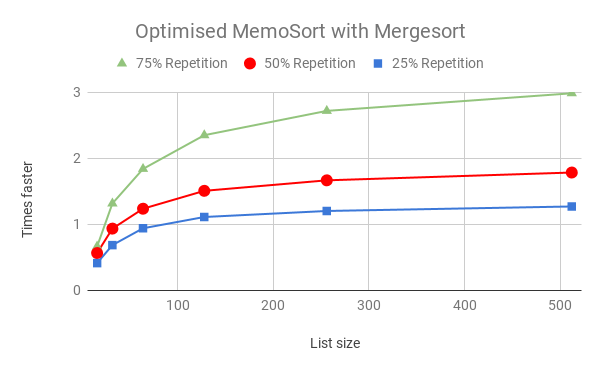
\includegraphics[height=8cm,keepaspectratio]{./images/OptMemoSortMerge.png}
    \caption{Times Optimised MemoSort is faster than brute force Mergesort}
    \label{fig:OptMemoSortMergeGraph}
\end{figure}


\begin{table}[H]
\centering
\begin{tabular}{|r|r|r|r|r|r|r|r|}   \hline
	{Length}  & {$100\%$} & {$75\%$} & {$50\%$} & {$25\%$} & {$0\%$} \\  \hline
	16 &1.857&0.668 & 0.569 &0.416&0.354\\ 
	32 &3.683&1.321 & 0.939&0.689&0.571\\ 
	64 &6.813 &1.845&1.241&0.945&0.762\\ 
	128 &10.011&2.357&1.513&1.116&0.888\\ 
	256 &13.736&2.726&1.672&1.207&0.947\\ 
	512 & 16.732&2.993&1.791&1.276&0.994\\  \hline
\end{tabular}
\caption{Optimised MemoSort speed factor using Mergesort with different repetitions}
\label{fig:OptMemoSortMergeTable}
\end{table}

\subsection{MemoBlockSort with 2-way-merge in similar lists}\label{MemoBlock2Res}

As discussed in section \ref{MemoBlockSort}, the overall performance of MemoBlockSort is not as good as MemoSort, even though a direct comparison can not be established as they focus on slightly different problems. \\

\begin{figure}[H]
\centering
\subcaptionbox{Insertionsort / 8 block size}{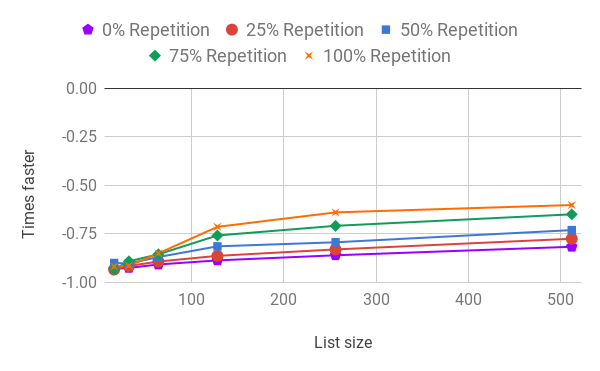
\includegraphics[height=5cm,keepaspectratio]{./images/2wayIns8.png}}%
\hfill % <-- Seperation
\subcaptionbox{Mergesort / 8 block size}{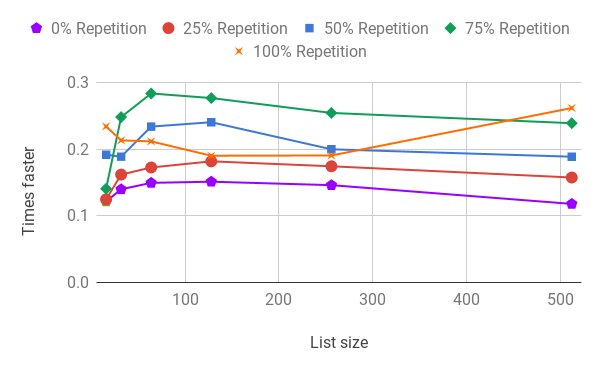
\includegraphics[height=5cm,keepaspectratio]{./images/2wayMerge8.png}}%
\\ % <-- Line break
\subcaptionbox{Insertionsort / 16 block size}{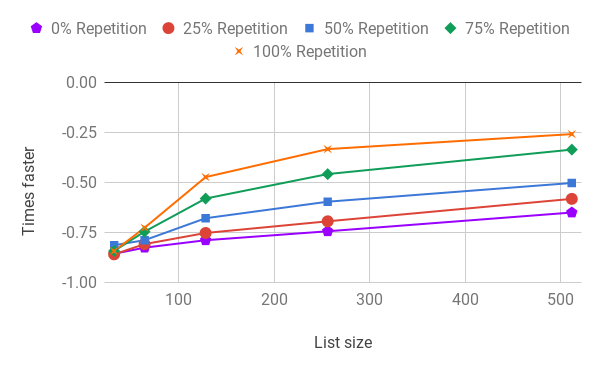
\includegraphics[height=5cm,keepaspectratio]{./images/2wayIns16.png}}%
\hfill % <-- Seperation
\subcaptionbox{Mergesort / 16 block size}{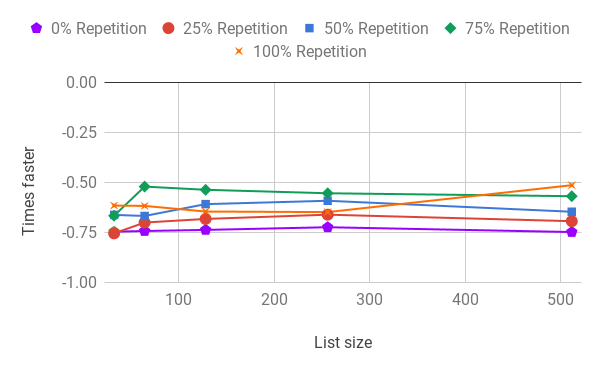
\includegraphics[height=5cm,keepaspectratio]{./images/2wayMerge16.png}}
\\ % <-- Line break
\subcaptionbox{Insertionsort / 64 block size}{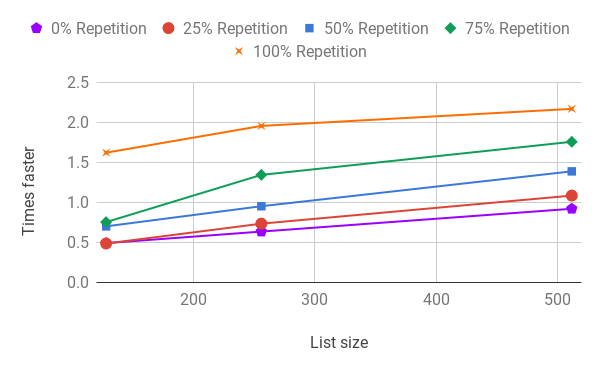
\includegraphics[height=5cm,keepaspectratio]{./images/2wayIns64.png}}%
\hfill % <-- Seperation
\subcaptionbox{Mergesort / 64 block size}{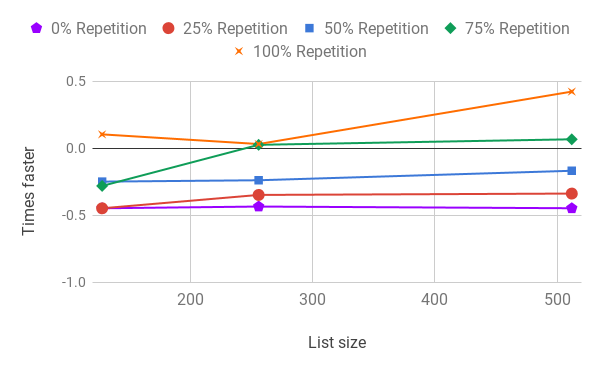
\includegraphics[height=5cm,keepaspectratio]{./images/2wayMerge64.png}}%
\caption{MemoBlockSort with 2-way merge performance}
\label{fig:MemoBlockSort2WayGraph}
\end{figure}

The overall overview of Figures \ref{fig:MemoBlockSort2WayGraph} (a) to (d), shows that for blocks of length 8 and 16 there is no real performance improvements, but for the 64 block size it was almost the only scenario where there was any improvement over brute force sorting, mainly in the version that uses Insertion sort. 
As a general trend, the higher the repetition and the bigger the list size the better time was achieved, mainly because for bigger list size the brute force approach takes more time than the overhead of using blocks plus the sorting avoided by the use of the memoization technique.

This can be viewed directly by comparing Figure \ref{fig:MemoBlockSort2WayGraph} (c) and (d), in which both Insertionsort and Mergesort MemoBlockSort have the same starting penalty with small list size and Insertionsort grows more steeply for bigger list size. This is explained because of the quadratic nature of Insertionsort for bigger size list, which allows for MemoBlockSort speed to comparatively be better. In contrast, MemoBlockSort with Mergesort maintains its penalty almost in a constant, because of the O(nlogn) time complexity of the brute force sorting all lists with merge sort.\\

Also by comparing the behaviour of MemoBlockSort with Insertionsort and MemoBlockSort with Mergesort, the Insertionsort approach has better performance in all scenarios. This is because the lists that are sorted have a small length of the blocks (purposely done for this study), and as it has been already proven in Figure \ref{fig:InsrtVsMerge}, Insertionsort performs better than Mergesort for this case of relatively short lists.\\


Finally in Figure \ref{fig:MemoBlockSort2WayGraph} (e) and (f)  it can be seen that this approach has better performance for Insertionsort when the block size is 64 and starting at 256 of list size and 50\% repetition. For Mergesort, the same is true but only after 75\% repetition.

\subsection{MemoBlockSort with k-way-merge in similar lists}

\begin{figure}[H]
\centering
\subcaptionbox{Insertionsort / 8 block size}{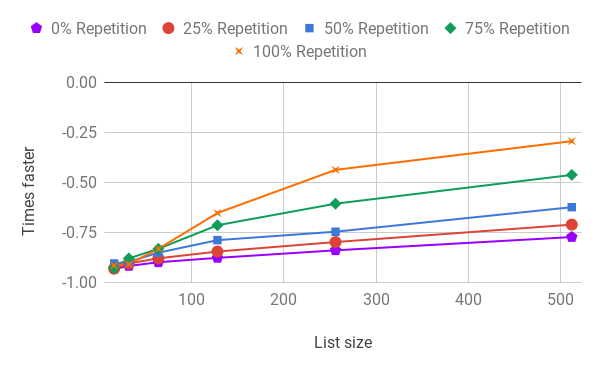
\includegraphics[height=5cm,keepaspectratio]{./images/kwayIns8.png}}%
\hfill % <-- Seperation
\subcaptionbox{Mergesort / 8 block size}{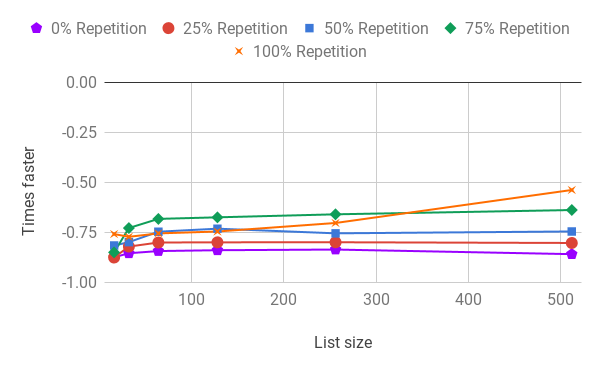
\includegraphics[height=5cm,keepaspectratio]{./images/kwayMerge8.png}}%
\\ % <-- Line break
\subcaptionbox{Insertionsort / 16 block size}{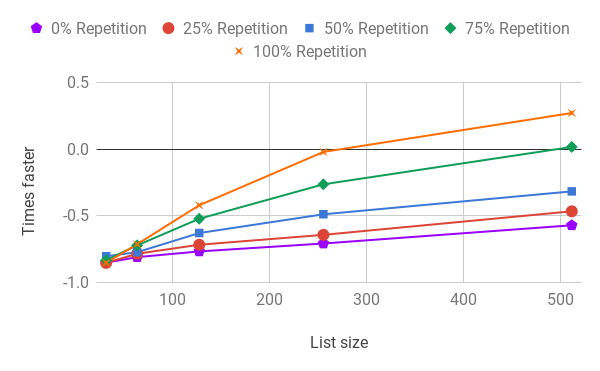
\includegraphics[height=5cm,keepaspectratio]{./images/kwayIns16.png}}%
\hfill % <-- Seperation
\subcaptionbox{Mergesort / 16 block size}{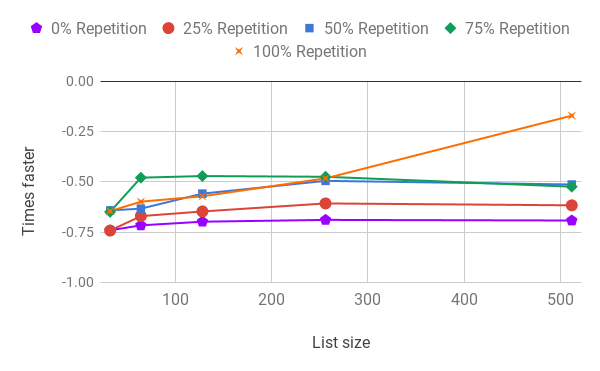
\includegraphics[height=5cm,keepaspectratio]{./images/kwayMerge16.png}}
\\ % <-- Line break
\subcaptionbox{Insertionsort / 64 block size}{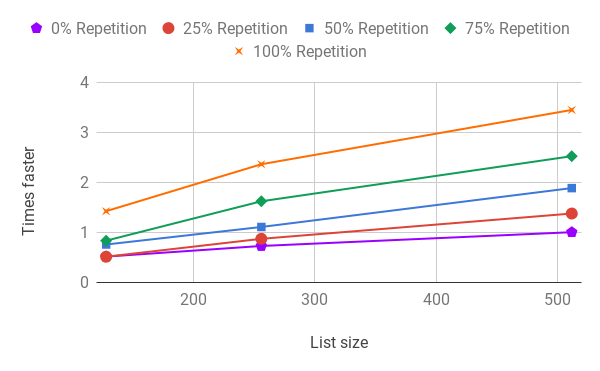
\includegraphics[height=5cm,keepaspectratio]{./images/kwayIns64.png}}%
\hfill % <-- Seperation
\subcaptionbox{Mergesort / 64 block size}{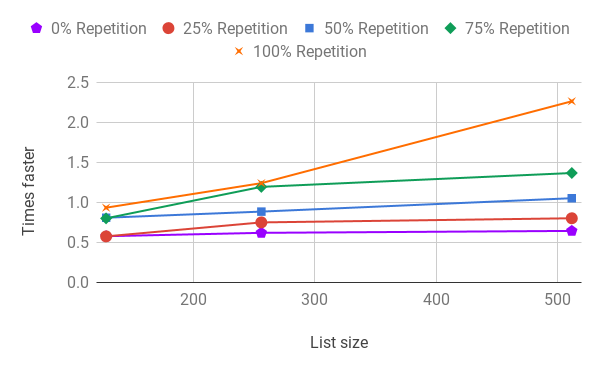
\includegraphics[height=5cm,keepaspectratio]{./images/kwayMerge64.png}}%
\caption{MemoBlockSort with k-way merge performance}
\label{fig:MemoBlockSortKWayGraph}
\end{figure}

The same analysis as in section \ref{MemoBlock2Res} is maintained here, except that with a k-way merge approach the algorithm behaves better. As Figure \ref{fig:MemoBlockSortKWayGraph} shows, there is a drastic improvement by just changing the way the algorithm merges the blocks. 
This confirms that for MemoBlockSort the real cost is not so much in the sorting algorithm as this only affects the sorting of each block, or the cost of the hashing function, but it  is more related to the reading and writing of blocks and the way they are managed.\\

Then it is clear that as displayed in Figure \ref{fig:MemoBlockSortKWayGraph} (e) and (f), this approach gives an improvement since the block size of 64 and from 256 list size onward and 50\% repetition, the same as 2-way merge approach, but performs much better.

\section{Conclusions}
The carried out study allowed us to model the behaviour of memoization techniques when sorting many similar lists of integer in different repetition scenarios. What we can conclude of this exercise is that the specific memoization technique utilised, the look  up table to find previous sorted lists, needs the definition of a hash function, a data structure to serve as a hash table and an algorithm to take advantage of the repetition.\\

What we found when looking for a suitable hash function for the study was that there are different kinds of hash function that can effectively work, just by providing a unique signature for a list of integers without collisions even with different approaches to calculate it but some are not necessarily the best fit for the use that we intended, as we showed that cryptographic functions do not perform well in this case, mainly because they were not design for speed performance as they perform multiple operation so it is hard to guess the probable result. Then we showed that a good fit hash function to use over a list of integers, in response to the research question RQ4 formulated in section \ref{researchQuestions}, could be either  {\it MurMur3}  or the proposed  {\it PairMultShift}, which both have a similar performance.\\

We also proposed a new approach to optimise sorting, {\it MemoSort} which applies the memoization technique to obtain a better performance than brute force sorting lists in different scenarios. We showed that this algorithm provides improvement up to 80 times when all list were the same, but in more realistic scenarios the performance improved according to the sorting algorithm, the length of the list and the repetition. Practically, it provided a slightly bigger improvement using Mergesort than Insertionsort as the sorting algorithm, although they behaved in a similar way. To answer RQ1 we then can summarise the finding in Table \ref{fig:MemoSortResults}.

\begin{table}[H]
\centering
\begin{tabular}{|c|p{70mm}|}   \hline
	{Sort Algorithm} & {Improvement} \\  \hline
	Insertionsort & 64 list size: 50\% repetition or more. 128 list size: 25\% repetition or more.\\ 
	Mergesort & 64 list size: 50\% repetition or more. 128 list size: 25\% repetition or more. \\  \hline
\end{tabular}
\caption{MemoSort results}
\label{fig:MemoSortResults}
\end{table}


We then showed a broader problem using memoization techniques when the repetition is between sub lists or blocks of the lists, it can also improve performance by introducing the {\it MemoBlockSort} algorithm. This algorithm did not prove to be so effective as {\it MemoSort}, but it allows for the problem to be broaden for different data scenario, also opening possibles applications on lists with different size.  It has however practical improvements for specific scenarios, which allows us to answer RQ2 with the findings summarised in Table \ref{fig:MemoBlockSortResults}.

\begin{table}[H]
\centering
\begin{tabular}{|c|r|p{80mm}|}  \hline
	{Sort Algorithm} & {Block size} & {Improvement} \\  \hline
	Insertionsort & 8 & No improvement. \\ 
	Insertionsort & 16 & Only improvement at 512 list size for 75\% repetition and above. \\ 
	Insertionsort & 64 & At  256 list size for 50\% repetition and above. For 512 list size, 25\% repetition and above.\\ 
	Mergesort & 8 &  No improvement. \\ 
	Mergesort & 16 & No improvement. \\ 
	Mergesort & 64 & At  256 list size for 75\% repetition and above. For 512 list size, 25\% repetition and above. \\  \hline
\end{tabular}
\caption{MemoBlockSort results}
\label{fig:MemoBlockSortResults}
\end{table}

This study also allowed us to conclude that Insertionsort even being a simple comparison sort, is one of the best algorithm to use in order to sort small lists, and its importance is sometimes overlooked but it must be kept in mind that it is part of the most used sorting algorithms, like Timsort and Introsort, both the standard sorting algorithms for popular languages as Java, Python, C\# and C++.

Finally, there was a chance of enhancing the proposed algorithms to get better results and answering question RQ4. We showed one possible approach for  {\it MemoSort} where the calculation of the signature is part of the operations in the sorting of the list. This approach did not improve the performance over {\it MemoSort}, but it did over brute force sorting the lists only for the case when sorting with Mergesort. \\

\section{Future Work}

While the objectives of this study serves as a initial exploration and they are reached by running the test cases with synthetic data, there is a need to find a suitable problem where the nature of the data fits the conclusions, so it can benefit of  the explored memoization techniques. The problem that served as inspiration \cite{Arch2015} is a possible candidate but some changes need to be done to fit the data of this problem, furthermore, some preliminary probing suggest that the data is not so repetitive to be able to benefit from the techniques studied.

Because the limitation on time of this study, there are multiple different improvements or alterations to be made to test the techniques in different scenarios, like exploring the behaviour with cache friendly version of the sorting algorithms and the merging process in {\it MemoBlockSort} and using the power of parallelisation by multi threading in CPU or by implementing memoization techniques in GPU sorting.

Also other memoization techniques can be constructed, like a probabilistic heuristic that samples elements of the lists between lists, instead of reading the whole list to match for previous sorted list.

For the specific problem on choosing the correct hash function, from the multiple implementations of hash functions, there may be faster one that is not universal but still have no collisions within the problems data and makes the memoization techniques more beneficial.

Other approaches to determine the similarities between list can be explored other than using a hash table, like local sensitive hashing, specifically the MinHash algorithm which can determine with a hash function the similar sets with a percentage of error.

\bibliographystyle{alpha}
% there are various bibliography styles you can set

\bibliography{references}


\section{Appendix}

\begin{table}[H]
\centering
\begin{tabular}{|r|r|r|r|r|r|r|r|}   \hline
	{Length} & {Insertionsort Only} & {$100\%$} & {$75\%$} & {$50\%$} & {$25\%$} & {$0\%$} \\  \hline
	16 &166 &169&373& 556& 666& 779\\ 
	32 &418 &194&443& 694& 868& 1,041\\ 
	64 &1,108&185 &1,639&1,021&1,416 & 1,740\\ 
	128 &3,005 &206&1,217&2,011&2,865 &3,667\\ 
	256 &8,943 &313&2,785&5,100&7,443&9,776\\ 
	512 &29,805& 360&8,078&15,59 &23,193 &30,742\\  \hline
\end{tabular}
\caption{MemoSort times (ms) using Insertionsort with different repetitions}
\end{table}

\begin{table}[H]
\centering
\begin{tabular}{|r|r|r|r|r|r|r|r|}   \hline
	{Length} & {Mergesort Only} & {$100\%$} & {$75\%$} & {$50\%$} & {$25\%$} & {$0\%$} \\  \hline
	16 &364&172&431 & 674 & 839 & 1,023\\ 
	32 &884&168&569 & 965& 1,258& 1,555\\ 
	64 &2,078&190 &931&1,569&2,144&2,759\\ 
	128 &4,705&228&1,625&2,903&4,183&5,439\\ 
	256 &10,632&303&3,205&6,081&8,750&11,568\\ 
	512 &23,709& 402&6,513&12,497&18,741&24,743\\  \hline
\end{tabular}
\caption{MemoSort times (ms) and speed factor using Mergesort with different repetitions}
\end{table}


\begin{table}[H]
\centering
\begin{tabular}{|r|r|r|r|r|r|r|r|}   \hline
	{Length} & {Insertionsort Only} & {$100\%$} & {$75\%$} & {$50\%$} & {$25\%$} & {$0\%$} \\  \hline
	16 &166&207&547 & 585 & 752 & 846\\ 
	32 &418&331&773 & 859& 1,034& 1,153\\ 
	64 &1,108&873 &1,523&1,617&1,783& 1,868\\ 
	128 &3,005&3,345&3,969&4,115&4,182 &4,243\\ 
	256 &8,943&11,870&12,376 &12,508&12,630&12,705\\ 
	512 &29,805 & 43,351&43,375 &43,625 &43,928 &43,782\\  \hline
\end{tabular}
\caption{Optimised MemoSort times (ms) using Insertionsort with different repetitions}
\end{table}

\begin{table}[H]
\centering
\begin{tabular}{|r|r|r|r|r|r|r|r|}   \hline
	{Length} & {Mergesort Only} & {$100\%$} & {$75\%$} & {$50\%$} & {$25\%$} & {$0\%$} \\  \hline
	16 &364&196&545 & 640 &874&1,028\\ 
	32 &884&240&669 & 941&1,283&1,548\\ 
	64 &2,078&305 &1,126&1,674&2,200&2,726\\ 
	128 &4,705&470&1,996&3,110&4,217&5,297\\ 
	256 &10,632&774&3,900&6,358&8,808&11,230\\ 
	512 &23,709& 1,417&7,921&13,241&18,588&23,864\\  \hline
\end{tabular}
\caption{Optimised MemoSort times (ms) using Mergesort with different repetitions}
\end{table}


%************* Aca abajo

\begin{table}[H]
\centering
\begin{tabular}{|r|r|r|r|r|}   \hline
	{List Length} & {Insertionsort Only} & {8} & {16} & {64} \\  \hline
	\multicolumn{5}{|l|}{ 0\% repetition} \\ \hline
	16 &166&2,392&- & - \\ 
	32 &412&5,473&2,869 & -\\ 
	64 &1,102&11,850 & 6,324 &-\\ 
	128 &2,988&26,200&14,136&6,068\\ 
	256 &8,820&62,840&34,440&13,856\\ 
	512 &29,397& 159,521&84,031&31,900\\  \hline
	\multicolumn{5}{|l|}{ 25\% repetition} \\ \hline
	16 &148&2,211&- & - \\ 
	32 &354&4,153&2,514 & -\\ 
	64 &951&18,796 & 4,952&-\\ 
	128 &2,706&19,694&10,927&5,555\\ 
	256 &8,331&48,859&27,228&11,327\\ 
	512 &28,648&127,027&68,511&26,368\\  \hline
	\multicolumn{5}{|l|}{ 50\% repetition} \\ \hline
	16 &117&1,166&- & - \\ 
	32 &287&2,921&1,539 & -\\ 
	64 &789&6,013 & 3,731&-\\ 
	128 &2,538&13,613&7,897&3,615\\ 
	256 &8,252&39,790&20,428&8,654\\ 
	512 &28,834&106,765&57,955&20,755\\  \hline
	\multicolumn{5}{|l|}{ 75\% repetition} \\ \hline
	16 &80&1,184&- & - \\ 
	32 &213&1,950&1,349 & -\\ 
	64 &638&4,385& 2,507&-\\ 
	128 &2,502&10,315&5,961&3,315\\ 
	256 &8,354&28,597&15,410&6,211\\ 
	512 &29,373&83,589&44,209&16,701\\  \hline
	\multicolumn{5}{|l|}{ 100\% repetition} \\ \hline
	16 &56&681&- & - \\ 
	32 &121&1,403&771 & -\\ 
	64 &500&3,328& 1,826&-\\ 
	128 &2,416&23,490&4,584&1,489\\ 
	256 &8,490&72,838&12,730&4,338\\ 
	512 &29,084&83,589&39,200&13,401\\  \hline
\end{tabular}
\caption{MemoBlockSort times (ms) using Insertionsort with 2-way merge for different list size, repetition and block sizes}
\end{table}


\begin{table}[H]
\centering
\begin{tabular}{|r|r|r|r|r|}   \hline
	{List Length} & {Mergesort Only} & {8} & {16} & {64} \\  \hline
	\multicolumn{5}{|l|}{ 0\% repetition} \\ \hline
	16 &355&2,919&- & - \\ 
	32 &886&6,338&3,487 & -\\ 
	64 &2,040&13,649 & 7,923 &-\\ 
	128 &4,636&30,665&17,629&8,369\\ 
	256 &10,446&71,544&37,802&18,432\\ 
	512 &23,208& 196,864&91,966&41,879\\  \hline
	\multicolumn{5}{|l|}{ 25\% repetition} \\ \hline
	16 &315&2,527&- & - \\ 
	32 &779&4,814&3,170 & -\\ 
	64 &1,814&10,516 & 6,052&-\\ 
	128 &4,177&22,984&13,142&7,544\\ 
	256 &9,647&55,345&28,446&14,762\\ 
	512 &22,250&141,289&72,566&33,528\\  \hline
	\multicolumn{5}{|l|}{ 50\% repetition} \\ \hline
	16 &251&1,310&- & - \\ 
	32 &631&3,344&1,866 & -\\ 
	64 &1,513&6,471 & 4,549&-\\ 
	128 &3,523&14,654&8,992&4,680\\ 
	256 &8,452&42,301&20,682&11,078\\ 
	512 &21,088&111,771&59,615&25,294\\  \hline
	\multicolumn{5}{|l|}{ 75\% repetition} \\ \hline
	16 &186&1,323&- & - \\ 
	32 &512&2,064&1534 & -\\ 
	64 &1,322&4,663& 2,757&-\\ 
	128 &2,976&10,757&6,420&4,130\\ 
	256 &7,393&29,069&16,570&7,196\\ 
	512 &20,192&84,507&46,794&18,895\\  \hline
	\multicolumn{5}{|l|}{ 100\% repetition} \\ \hline
	16 &158&675&- & - \\ 
	32 &297&1,393&772 & -\\ 
	64 &684&3,232& 1786&-\\ 
	128 &1,584&8,330&4465&1,433\\ 
	256 &19,067&23,552&12,746&4,343\\ 
	512 &4,487&72,868&39,184&13,386\\  \hline
\end{tabular}
\caption{MemoBlockSort times (ms) using Mergesort with 2-way merge for different list size, repetition and block sizes}
\end{table}


\begin{table}[H]
\centering
\begin{tabular}{|r|r|r|r|r|}   \hline
	{List Length} & {Insertionsort Only} & {8} & {16} & {64} \\  \hline
	\multicolumn{5}{|l|}{ 0\% repetition} \\ \hline
	16 &166&2,450&- & - \\ 
	32 &412&4,977&2,771 & -\\ 
	64 &1,102&10,870 & 5,794 &-\\ 
	128 &2,988&24,258&12,814&5,768\\ 
	256 &8,820&54,812&30,156&12,072\\ 
	512 &29,397& 129,365&68,504&29,213\\  \hline
	\multicolumn{5}{|l|}{ 25\% repetition} \\ \hline
	16 &148&2,141&- & - \\ 
	32 &354&37,03&2,407 & -\\ 
	64 &951&7,866 & 4,406&-\\ 
	128 &2,706&17,487&9,558&5,248\\ 
	256 &8,331&41,189&23,308&9,534\\ 
	512 &28,648&98,972&53,653&20,770\\  \hline
	\multicolumn{5}{|l|}{ 50\% repetition} \\ \hline
	16 &80&1,227&- & - \\ 
	32 &213&2,771&1,459 & -\\ 
	64 &638&5,290& 3,470&-\\ 
	128 &2,502&11,984&6,841&3,340\\ 
	256 &8,354&32,489&16,132&7,430\\ 
	512 &29,373&76,570&42,189&15,269\\  \hline
	\multicolumn{5}{|l|}{ 75\% repetition} \\ \hline
	16 &56&1,121&- & - \\ 
	32 &121&1,767&1,273 & -\\ 
	64 &500&3,786& 2,291&-\\ 
	128 &2,416&8,740&5,234&2,991\\ 
	256 &8,490&2,1201&11,344&5,143\\ 
	512 &29,084&54,604&28,898&11,628\\  \hline
	\multicolumn{5}{|l|}{ 100\% repetition} \\ \hline
	16 &56&1,312&- & - \\ 
	32 &121&2,973&820 & -\\ 
	64 &500&3,786& 1,740&-\\ 
	128 &2,416&6,955&4,171&1,694\\ 
	256 &8,490&15,073&8,671&3,590\\ 
	512 &29,084&41,164&22,880&8,428\\  \hline
\end{tabular}
\caption{MemoBlockSort times (ms) using Insertionsort with K-way merge for different list size, repetition and block sizes}
\end{table}


\begin{table}[H]
\centering
\begin{tabular}{|r|r|r|r|r|}   \hline
	{List Length} & {Mergesort Only} & {8} & {16} & {64} \\  \hline
	\multicolumn{5}{|l|}{ 0\% repetition} \\ \hline
	16 &355&2,816&- & - \\ 
	32 &886&6,054&3,413 & -\\ 
	64 &2,040&12,975 & 7,174 &-\\ 
	128 &4,636&28,716&15,325&8,012\\ 
	256 &10,446&63,393&33,540&16,828\\ 
	512 &23,208& 16,3679&75,246&35,984\\  \hline
	\multicolumn{5}{|l|}{ 25\% repetition} \\ \hline
	16 &315&2,522&- & - \\ 
	32 &779&4,337&3,015 & -\\ 
	64 &1,814&9,071 & 5,495&-\\ 
	128 &4,177&20,792&11,817&7,245\\ 
	256 &9,647&47,935&24,524&12,842\\ 
	512 &22,250&112,567&57,945&27,712\\  \hline
	\multicolumn{5}{|l|}{ 50\% repetition} \\ \hline
	16 &251&1,358&- & - \\ 
	32 &631&31,27&1,759 & -\\ 
	64 &1,513&5,957 & 4,119&-\\ 
	128 &3,523&13,092&7,968&4,351\\ 
	256 &8,452&34,378&16,714&9,537\\ 
	512 &21,088&82,630&43,253&20,017\\  \hline
	\multicolumn{5}{|l|}{ 75\% repetition} \\ \hline
	16 &186&1,233&- & - \\ 
	32 &512&1,880&1,457 & -\\ 
	64 &1,322&4,156& 2,535&-\\ 
	128 &2,976&9,133&5,620&3,711\\ 
	256 &7,393&21,686&14,056&6,185\\ 
	512 &20,192&55,729&42,367&14,754\\  \hline
	\multicolumn{5}{|l|}{ 100\% repetition} \\ \hline
	16 &158&652&- & - \\ 
	32 &297&1,300&837 & -\\ 
	64 &684&2,786& 1,701&-\\ 
	128 &1,584&6,212&3,692&1,694\\ 
	256 &19,067&15,078&8,662&3,614\\ 
	512 &4,487&41,221&22,974&8,418\\  \hline
\end{tabular}
\caption{MemoBlockSort times (ms) using Mergesort with K-way merge for different list size, repetition and block sizes}
\end{table}





\end{document}
